\documentclass[a4paper,12pt]{article}
\usepackage[utf8]{inputenc}
\usepackage[T1]{fontenc}
\usepackage[english]{babel}
\usepackage{graphicx}
\usepackage{booktabs}
\usepackage{amsmath}
\usepackage{hyperref}
\usepackage{geometry}
\usepackage{listings}
\usepackage{wrapfig}
\usepackage{float} 
\geometry{a4paper, margin=1in}
\title{From Chest X-rays to Medical Reports: A Deep Learning Approach}
\author{Frandina Ilaria 264232 \quad Siciliano Samuele 263633 \quad Spadafora Pierpaolo 263722}
\date{}
\begin{document}
\maketitle

\section{Introduction}
In this report, we present a comprehensive multi-task deep learning approach for chest X-ray analysis. Our goal is to develop a unified model that simultaneously performs disease classification, radiological report generation, and image reconstruction.

The model leverages state-of-the-art architectures by combining ResNet-based encoders for extracting image features, GPT-2 for generating textual reports, and a Variational Autoencoder (VAE) for reconstructing input images. This integration improves the interpretability of the diagnostic process while ensuring that the learned representations remain robust and clinically relevant.

To achieve this, we first implemented a rigorous data cleaning pipeline to ensure high-quality inputs by filtering out incomplete or low-quality reports and images. The resulting dataset includes both frontal and lateral X-ray views, each accompanied by detailed clinical findings.

Our multi-task model is trained end-to-end with a composite loss function that integrates classification loss (augmented with focal loss to address class imbalance), caption generation loss (using teacher forcing techniques), and VAE reconstruction loss (MSE and KLD). We evaluate the model using classification accuracy, BLEU, and ROUGE scores across different tasks.

\section{Dataset Description}
The initial dataset consisted of:
\begin{itemize}
    \item A collection of frontal and lateral X-ray images.
    \item Two CSV files containing, respectively, the projection information of the images and the associated reports (including clinical findings and pathologies).
\end{itemize}

\begin{table}[H]
\centering
\begin{tabular}{l c}
\toprule
\textbf{Item} & \textbf{Value} \\
\midrule
Total number of UIDs & 2728 \\
Number of Validated Reports & 5574 \\
Number of Images Used & 5574 (2728 per view) \\
\bottomrule
\end{tabular}
\caption{Initial Dataset Statistics}
\label{tab:dataset_stats}
\end{table}

\section{Data Preprocessing and Cleaning}
To ensure data quality and reduce potential noise during training, we performed the following steps:
\begin{enumerate}
    \item \textbf{Elimination of Incomplete Records:}  
    \begin{itemize}
        \item All records with one or more essential fields (e.g., \texttt{findings}, \texttt{Problems}, \texttt{MeSH}) that were empty or contained only blank strings were removed.
    \end{itemize}
    \item \textbf{Verification of Image Consistency:}  
    \begin{itemize}
        \item Records that did not contain exactly one frontal and one lateral X-ray were excluded to guarantee the presence of both views for each UID.
    \end{itemize}
    \item \textbf{Filtering Based on Pathology Frequency:}  
    \begin{itemize}
        \item Pathologies whose total occurrences did not exceed a threshold (in this case, 20) were discarded.
    \end{itemize}
    \item \textbf{Grouping into Macro-categories:}  
    \begin{itemize}
        \item Pathologies were grouped into macro-categories. The categorization was adapted based on the type of classification:
        \begin{itemize}
            \item \textbf{Binary:} pathology vs. no pathology.
            \item \textbf{Ternary:} pulmonary problems versus other issues.
            \item \textbf{Multiclass:} division into 5 (or more) categories.
        \end{itemize}
    \end{itemize}
\end{enumerate}

It should be noted that due to the intrinsic nature of the dataset (X-rays), conventional data augmentation techniques could not be applied effectively. For instance, a simple horizontal flip would reverse the positions of the organs, potentially introducing errors and misleading conclusions.

\section{Dataset Splitting and DataLoaders}
After cleaning, the dataset was split as follows:
\begin{itemize}
    \item \textbf{Training set:} 60\%
    \item \textbf{Validation set:} 20\%
    \item \textbf{Test set:} 20\%
\end{itemize}
To simplify loading data onto the GPU and to concatenate the images (frontal and lateral) with the textual reports, a custom \texttt{Dataset} class (based on \texttt{torch.utils.data.Dataset}) was implemented. Corresponding DataLoaders were then created for training, validation, and testing.

\section{Model Architecture}
The proposed model, \textit{AllegroChirurgoModel}, integrates several components:

\subsection{Image Encoders}
\begin{itemize}
    \item A pre-trained \textbf{ResNet50} is used for each view (frontal and lateral).
    \item The final layer is replaced with an identity layer (\texttt{nn.Identity}) to extract features.
    \item Most of the ResNet50 layers are frozen, leaving only the last 6 layers trainable to allow fine-tuning during training.
\end{itemize}

\subsection{Classification Branch}
The features extracted from the two ResNets are:
\begin{itemize}
    \item Concatenated and passed through several fully connected layers (with dropout and layer normalization) to obtain the final classification logits.
    \item The classification loss is computed using \textbf{Cross-Entropy Loss} (and, where necessary, \textbf{Focal Loss} to address underrepresented classes).
\end{itemize}

\subsection{Report Generation Decoder}
\begin{itemize}
    \item The combined features are projected into a space with a dimension compatible with the decoder input (GPT-2 uses embeddings of dimension 768, while the feature vector extracted from ResNet is 2048).
    \item The decoder is based on \textbf{GPT-2 LMHeadModel}, which is adapted by resizing the vocabulary based on the tokenizer used.
    \item Teacher forcing is employed during training to improve the quality of report generation.
\end{itemize}

\subsection{VAE Branch for Image Reconstruction}
\begin{itemize}
    \item From the combined feature vector, the parameters $\mu$ and $\log\sigma^2$ are extracted for the \textbf{reparameterization trick}.
    \item A fully connected layer projects the latent vector into a dimension that is then "deconvolved" using a series of \textbf{ConvTranspose2d} layers to reconstruct both the frontal and lateral images.
    \item The VAE loss is calculated as the sum of the \textbf{Mean Squared Error (MSE)} for reconstruction and the \textbf{Kullback-Leibler Divergence (KLD)}.
\end{itemize}

\section{Training and Evaluation Process}
In our initial approach, the following components were optimized simultaneously during training:
\begin{itemize}
    \item \textbf{Classification Loss:} Computed on the logits from the classification branch.
    \item \textbf{Report Generation Loss:} Using the GPT-2 decoder, the loss is computed by comparing the generated sequences with the ground truth.
    \item \textbf{VAE Loss:} A combination of reconstruction loss and KLD.
\end{itemize}
The total loss function is a linear combination of these components, weighted by the coefficients \texttt{ALPHA\_MAIN\_MODEL} (for the caption loss) and \texttt{BETA\_VAE} (for the VAE loss). For training, we employed:
\begin{itemize}
    \item A \textbf{Scheduler} to reduce the learning rate upon plateau.
    \item \textbf{Early Stopping} to halt training when no improvements in validation loss are observed.
\end{itemize}
Evaluation metrics include:
\begin{itemize}
    \item \textbf{Accuracy} for classification.
    \item \textbf{BLEU} and \textbf{ROUGE-L} scores to assess the quality of the generated reports.
\end{itemize}

\begin{figure}[H]
\centering
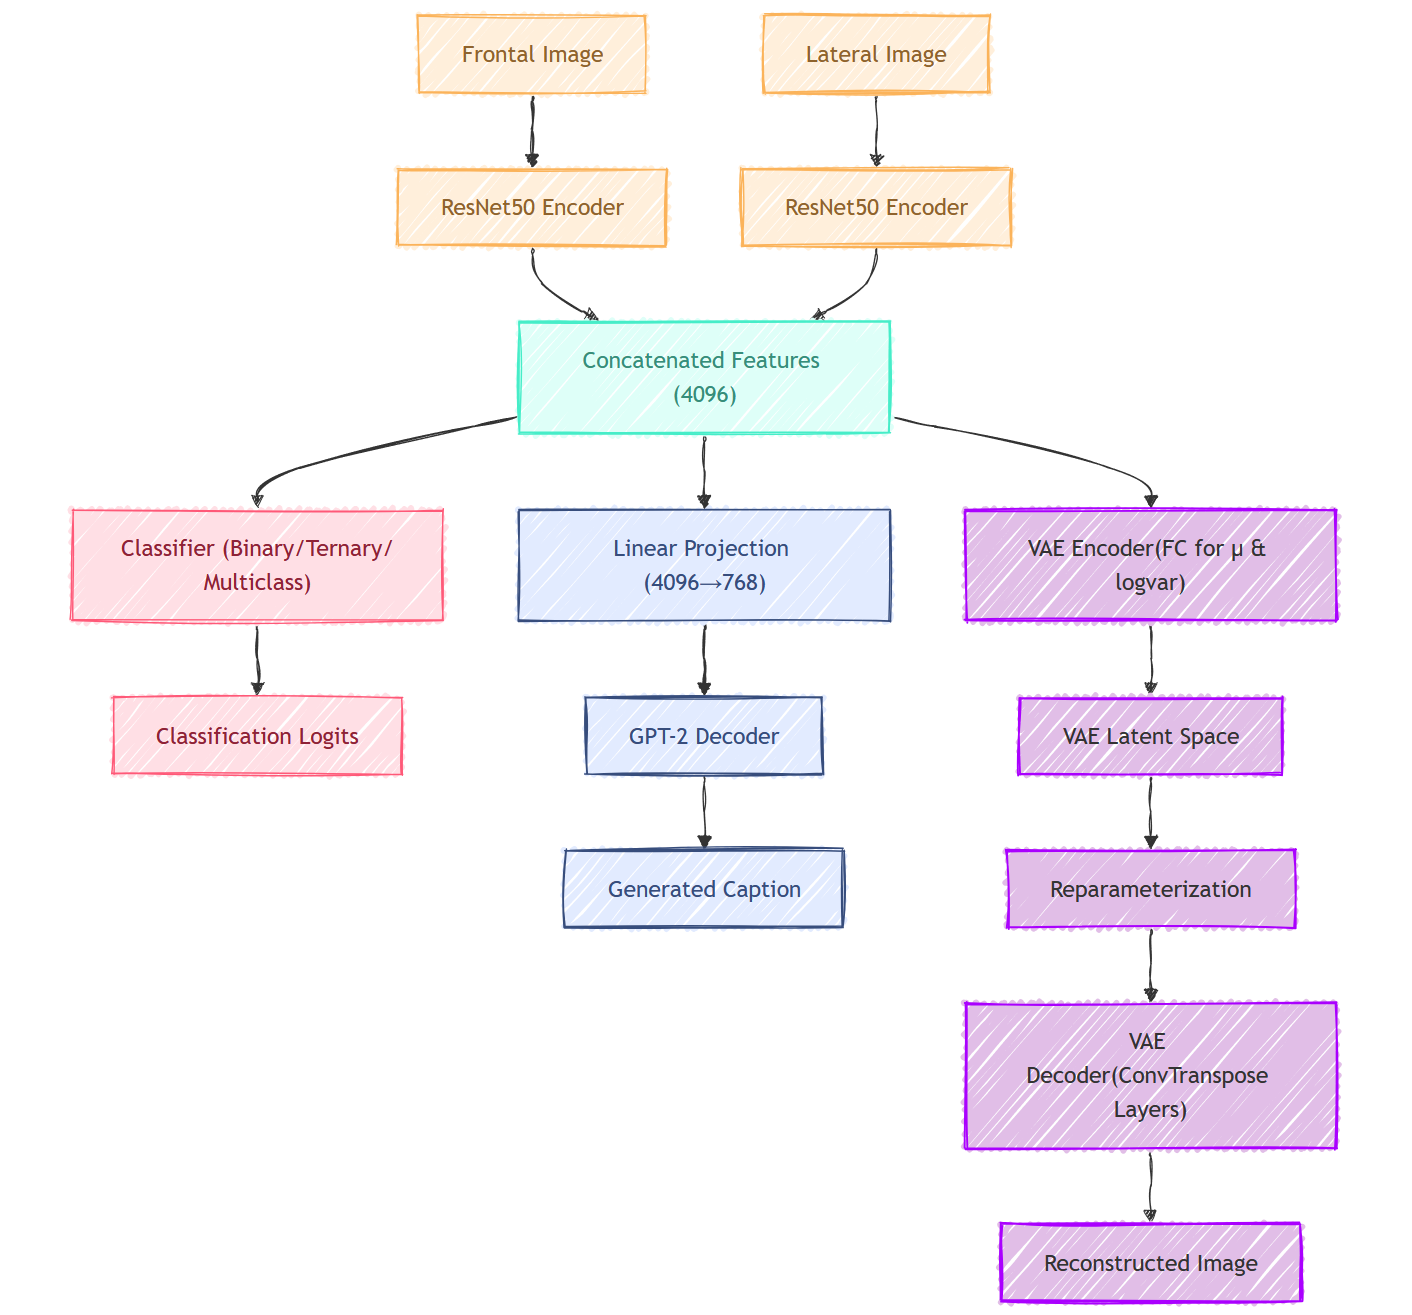
\includegraphics[width=0.8\linewidth]{./Grafici/Completo_Tutto_Unito.png}
\caption{Overall training and evaluation pipeline.}
\label{fig:complete_pipeline}
\end{figure}

This approach enabled us to develop a model capable of providing both diagnosis and report generation from the same latent space.\\
However, it became evident that combining multiple tasks into a single model, especially with an insufficient amount of data, led to less than satisfactory results.

We implemented Focal Loss to mitigate the issue of underrepresented classes in the classification task and adjusted the weighting of the losses, reducing the impact of both the text prediction and the VAE losses.\\

For the training process, we implemented two key optimization strategies:

\begin{itemize}
    \item A \textbf{Learning Rate Scheduler (ReduceLROnPlateau)} that monitors the validation loss and reduces the learning rate by a factor of 0.5 if no improvement is observed for 2 consecutive epochs. 
    This helps the model converge to better local minima when the training process starts to plateau.
    
    \item An \textbf{Early Stopping} mechanism that tracks the validation loss and stops the training if no improvement is detected for 3 consecutive epochs. 
    This, along with dropout in the classifier network, prevents overfitting and ensures optimal model performance while saving computational resources.
\end{itemize}


Despite these measures, we observed that the model's accuracy in the binary classification scenario fell below 70\%, with significant challenges in generating accurate text and faithfully reconstructing images.\\

\begin{quote}
    \textbf{True Caption:}\\
    The cardiac contours are normal. The lungs are clear. Thoracic spondylosis.
    
    \medskip
    
    \textbf{Pred Caption (Model Output):}\\
    The heart and lungs have XXXX XXXX in the interval. Both lungs are clear and expanded. 
    No pleural air collections. Heart and mediastinum normal.
\end{quote}
    
\begin{table}[H]
    \centering
    \begin{tabular}{lccccccc}
    \toprule
     & \textbf{Class 1} & \textbf{Class 2} & \textbf{Class 3} & \textbf{Class 4} & \textbf{Class 5} & \textbf{Total Accuracy} \\
    \midrule
    \textbf{Binary} & 61.46\% & 68.33\% & - & - & - & 65.75\% \\
    \textbf{Ternary} & 15.12\% & 68.20\% & 39.52\% & - & - & 41.76\% \\ 
    \textbf{Multiclass} & 38.54\% & 8.29\% & 14.71\% & 41.30\% & 34.09\% & 24.91\% \\
    \bottomrule
    \end{tabular}
    \caption{Classification and Text Generation Results}
    \label{tab:classification_textgen_results}
\end{table}
\begin{table}[H]
    \centering
    \begin{tabular}{lccccccc}
    \toprule
     & \textbf{BLEU-1} & \textbf{BLEU-2} & \textbf{BLEU-3} & \textbf{BLEU-4} & \textbf{ROUGE-L} \\
    \midrule
    \textbf{Binary} & 0.0795 & 0.0625 & 0.0523 & 0.0442 & 0.2427 \\
    \textbf{Ternary} & 0.0830 & 0.0640 & 0.0526 & 0.0436 & 0.2564 \\
    \textbf{Multiclass}  & 0.0781 & 0.0616 & 0.0515 & 0.0435 & 0.2517 \\
    \bottomrule
    \end{tabular}
    \caption{Classification and Text Generation Results}
    \label{tab:classification_textgen_results}
\end{table}
    
\begin{figure}[H]
    \centering
    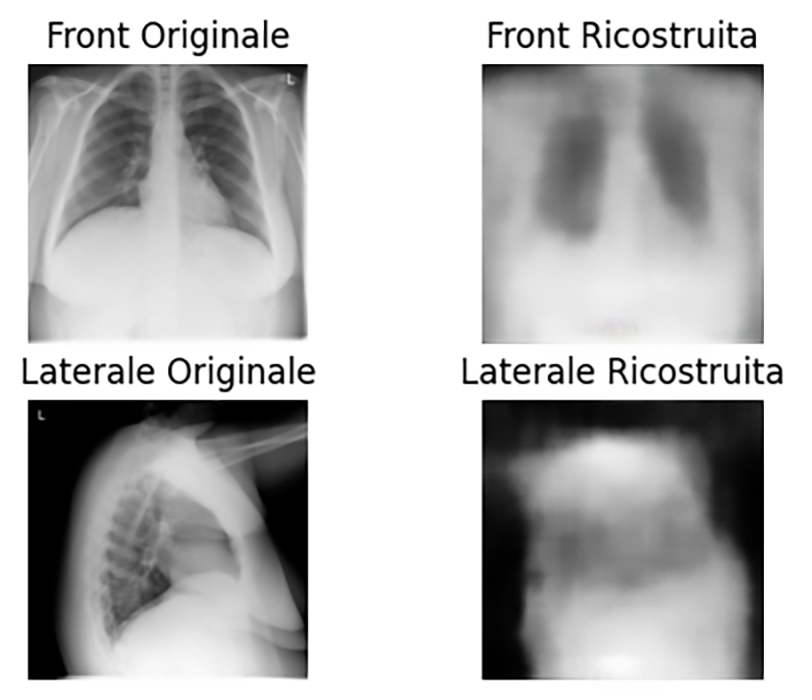
\includegraphics[width=0.5\linewidth]{./Grafici/UNITO_IMAGE_RECONSTRUCTION.png}
    \caption{Examples of image reconstructions.}
    \label{fig:image_recon}
\end{figure}

To address these issues, we modified our approach by separating the tasks into two distinct models: 
\begin{enumerate}
    \item \textbf{AllegroChirurgoModel} for classification and report generation.
    \item \textbf{VAEModel} for image reconstruction.
\end{enumerate} 
aiming to isolate the challenges and better understand the sources of errors.

\begin{figure}[H]
    \centering
    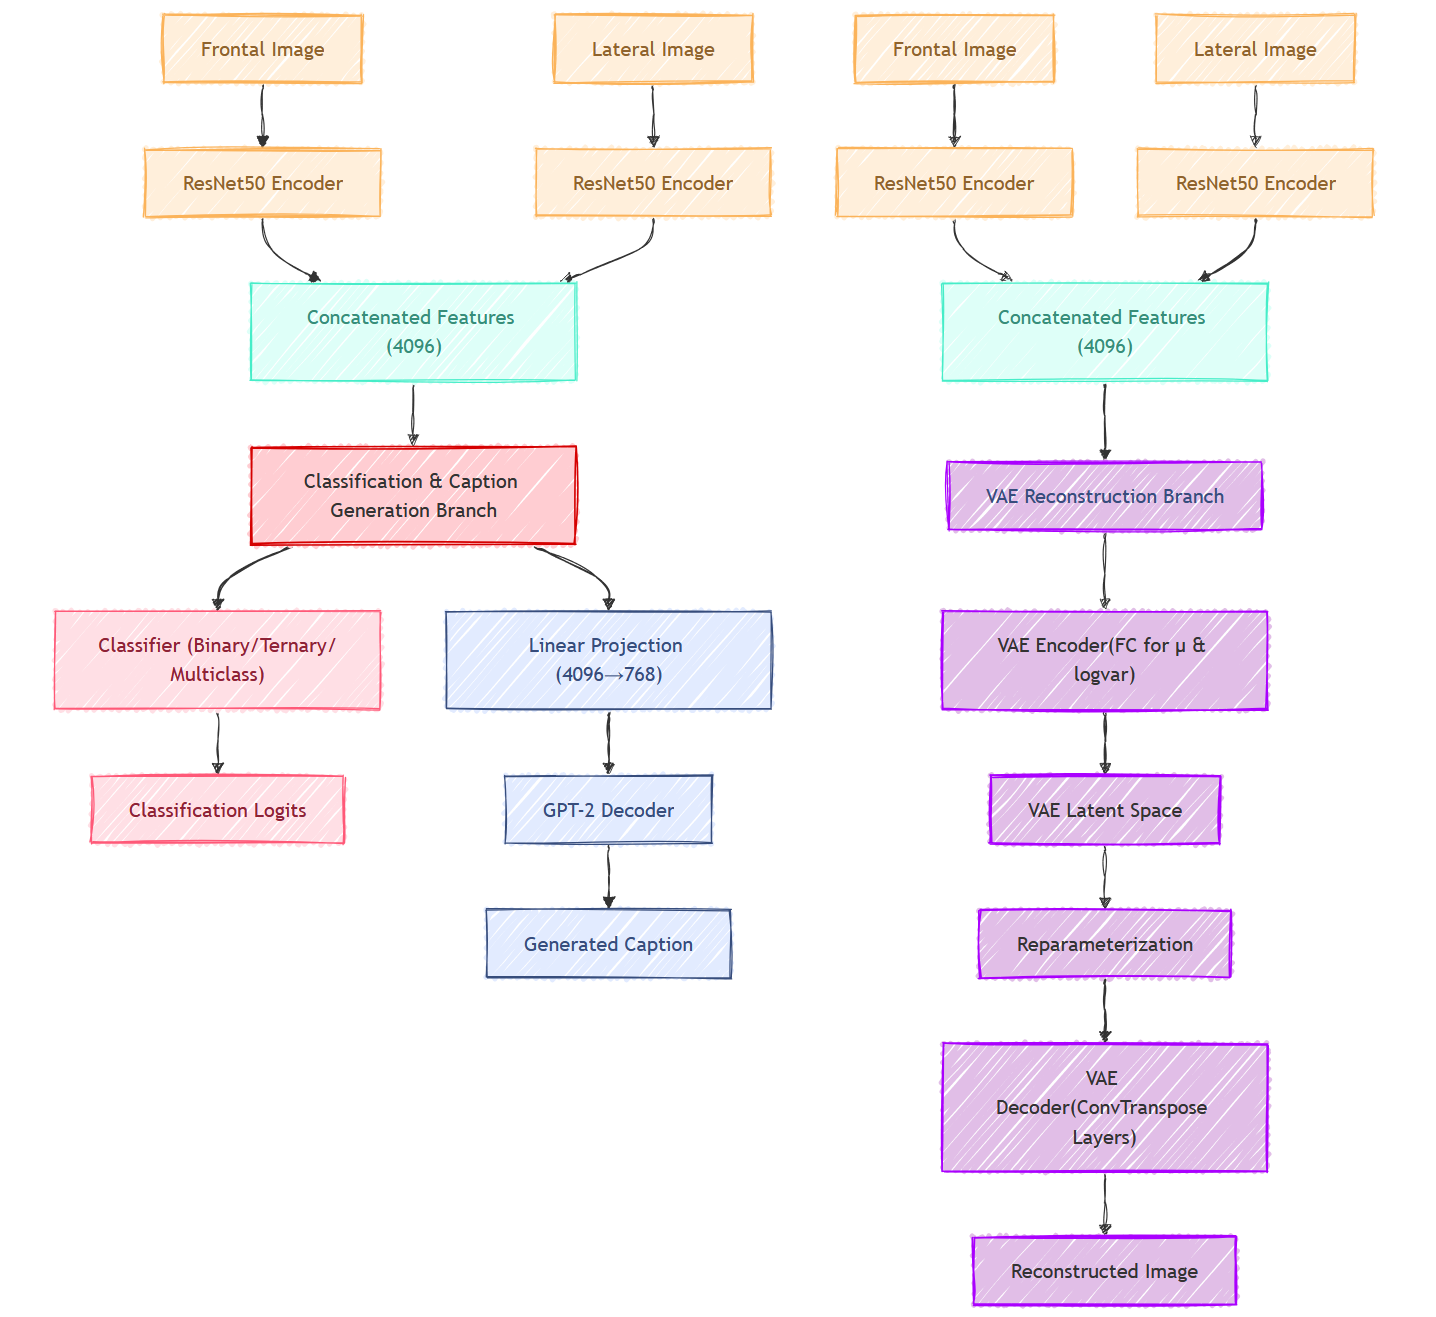
\includegraphics[width=0.8\linewidth]{./Grafici/Completo_Vae_Separato.png}
    \caption{Architecture for the classification and caption generation model.}
    \label{fig:classifier_caption}
\end{figure}


\subsection{Results with the Separated Architecture}
This new architecture allowed us to obtain better results, maintaining a similar (or slightly higher) classification accuracy—especially in multi-class scenarios, where the previous model's accuracy approached zero for almost all classes—and improving text generation by significantly boosting BLEU scores and reducing meaningless word generation.\\

Additionally, the VAE model showed enhanced image reconstruction quality. However, this objective remains less significant when combined with the necessity of unifying all three branches in a single model.

\begin{quote}
    \textbf{True Caption:}\\
    The cardiac contours are normal. The lungs are clear. Thoracic spondylosis.
    
    \medskip
    
    \textbf{Pred Caption (Model Output):}\\
    The cardiac silhouette is within normal limits for appearance in the contour of the frontal XXXX. No focal area of pulmonary consolidation is identified. No pneumothorax or effusion is identified.
\end{quote}

\begin{table}[H]
    \centering
    \begin{tabular}{lccccccc}
    \toprule
     & \textbf{Class 1} & \textbf{Class 2} & \textbf{Class 3} & \textbf{Class 4} & \textbf{Class 5} & \textbf{Total Accuracy} \\
    \midrule
    \textbf{Binary} & 74.63\% & 67.45\% & - & - & - & 70.73\% \\
    \textbf{Ternary} & 49.27\% & 58.53\% & 37.90\% & - & - & 50.37\% \\
    \textbf{Multiclass} & 70.73\% & 6.67\% & 54.32\% & 25.27 \% & 12.77\% & 41.94\% \\
    \bottomrule
    \end{tabular}
    \caption{Classification and Text Generation Results}
    \label{tab:classification_textgen_results}
\end{table}
\begin{table}[H]
    \centering
    \begin{tabular}{lccccccc}
    \toprule
     & \textbf{BLEU-1} & \textbf{BLEU-2} & \textbf{BLEU-3} & \textbf{BLEU-4} & \textbf{ROUGE-L} \\
    \midrule
    \textbf{Binary} & 0.2649 & 0.2369 & 0.2207 & 0.2067 & 0.2375 \\
    \textbf{Ternary} & 0.2900 & 0.2639 & 0.2485 & 0.2352 & 0.2410 \\
    \textbf{Multiclass}  & 0.2109 & 0.1865 & 0.1724 & 0.1606 & 0.2334 \\
    \bottomrule
    \end{tabular}
    \caption{Classification and Text Generation Results}
    \label{tab:classification_textgen_results}
\end{table}
    
\begin{figure}[H]
    \centering
    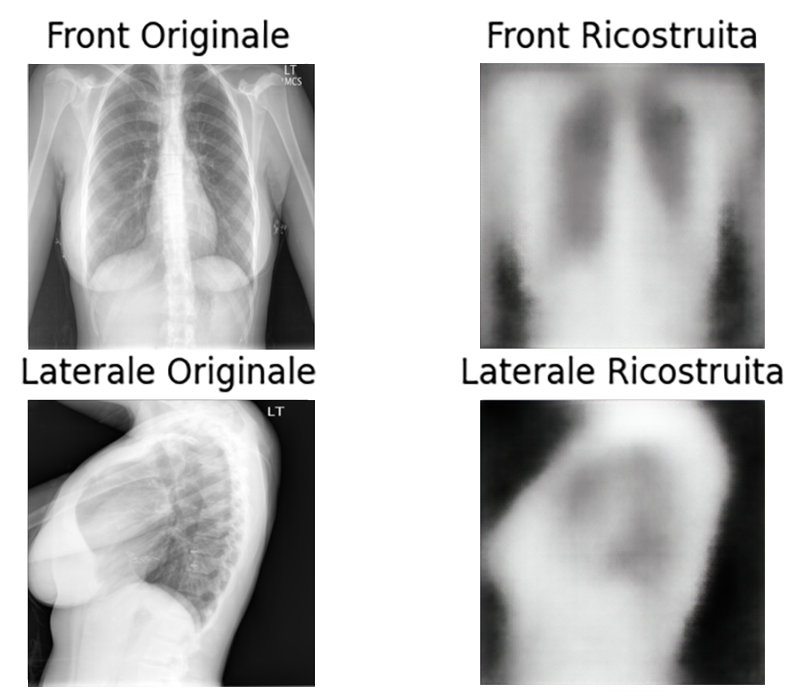
\includegraphics[width=0.6\linewidth]{./Grafici/IMAGE_RECONSTRUCTION.png}
    \caption{Examples of image reconstructions.}
    \label{fig:image_recon}
    \end{figure}



From these tables, it is evident that multi-class models—due to having many underrepresented classes—generally incur a more significant classification loss. This loss heavily impacts the latent space, leading to substantially worse results overall.

\subsection{Architecture with the Custom Transformer}
\begin{wrapfigure}{R}{0.5\textwidth}
    \centering
    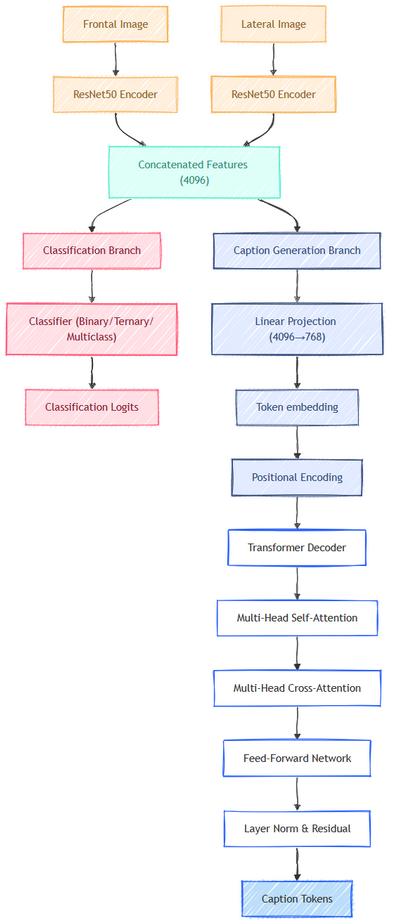
\includegraphics[width=0.95\linewidth]{./Grafici/Completo_Tutto_Architettura_Custom}
    \caption{Architecture for the classification and caption generation model.}
    \label{fig:custom_transformer}
\end{wrapfigure}

We also tried an architecture with a \textbf{Custom Transformer} that draws inspiration from the GPT-2 architecture but implements a lighter, more flexible design. 
This choice offers direct control over the model's structure and core components:

\begin{enumerate}
    \item We apply a custom \textbf{Positional Encoding} to the \textit{input embeddings} to provide the model with information about the position of tokens in the sequence. This is essential for the Transformer to keep track of word order and capture relationships between distant tokens.

    \item \textbf{Transformer Encoder:}  
    This module leverages the \textit{self-attention} mechanism to weigh the importance of different tokens during prediction, while the \textit{feed-forward network} further processes the information coming out of the self-attention layer. During training, we apply \textit{sub-sequence masking} to prevent the model from "seeing" future tokens and to learn how to predict the next word based solely on the preceding context.

    \item The \textbf{Forward Method} processes the input tokens in order by passing them through:
    \begin{itemize}
        \item An embedding layer.
        \item The positional encoding layer.
        \item The \textit{Transformer Encoder} block (which can be repeated multiple times, depending on the chosen depth).
    \end{itemize}
    The output of the Transformer Encoder is then fed into a linear layer (\texttt{nn.Linear}) to predict the next token in the sequence.

    \item During \textbf{Generation} the model predicts tokens one at a time, based on all previously generated tokens. Each predicted token is appended to the input sequence, and this process continues until an end-of-sequence token (e.g., \texttt{<EOS>}) is produced or a predefined maximum length is reached.
\end{enumerate}

\indent
Our goal is to provide a more modular approach compared to GPT-2, while retaining the benefits of an attention mechanism that models long-range relationships. This design allowed us to experiment with various configurations of \textit{layers}, \textit{heads}, and embedding sizes, ultimately finding a good balance between generalization capability and computational efficiency.

\begin{quote}
    \textbf{True Caption:}\\
    The cardiac contours are normal. The lungs are clear. Thoracic spondylosis.
    
    \medskip
    
    \textbf{Pred Caption (Model Output):}\\
    cardiomediastinal silhouette and hilar contours. Lungs are clear without focal consolidation, pneumothorax, large pleural effusion, or pneumothorax. Cardiomediastinal contours are unremarkable. Negative for acute bony findings. Stable degenerative changes of the thoracic spine. No XXXX. Stable mild degenerative changes of the thoracic spine. Degenerative changes noted within the thoracic spine. Visualized skeletal structures are within the thoracic spine. Calcified right. Stable cardiaphragm. Stable normal limits.
\end{quote}

\newpage

\begin{table}[H]
    \centering
    \begin{tabular}{lccccccc}
    \toprule
     & \textbf{Class 1} & \textbf{Class 2} & \textbf{Class 3} & \textbf{Class 4} & \textbf{Class 5} & \textbf{Total Accuracy} \\
    \midrule
    \textbf{Binary}         & 80.00\% & 61.29\% & - & - & - & 68.32\% \\ 
    \textbf{Ternary}        & 33.17\% & 61.75\% & 45.97\% & - & - & 47.44\% \\ 
    \textbf{Multiclass}     & 63.90\% & 17.74\% & 15.38\% & 8.51\% & 19.11\% & 34.62\% \\ 
    \bottomrule
    \end{tabular}
    \caption{Classification and Text Generation Results}
    \label{tab:classification_textgen_results}
\end{table}
\begin{table}[H]
    \centering
    \begin{tabular}{lccccccc}
    \toprule
     & \textbf{BLEU-1} & \textbf{BLEU-2} & \textbf{BLEU-3} & \textbf{BLEU-4} & \textbf{ROUGE-L} \\
    \midrule
    \textbf{Binary}         & 0.2074 & 0.1468 & 0.1093 & 0.0782 & 0.1875 \\
    \textbf{Ternary}        & 0.1981 & 0.1398 & 0.1045 & 0.0757 & 0.1767 \\
    \textbf{Multiclass}     & 0.2019 & 0.1407 & 0.1039 & 0.0735 & 0.1790 \\
    \bottomrule
    \end{tabular}
    \caption{Classification and Text Generation Results}
    \label{tab:classification_textgen_results}
\end{table}

\begin{wrapfigure}{R}{1\textwidth}
    \section{Conclusions}

    In this work, we presented a comprehensive investigation of multi-task deep learning approaches for chest X-ray analysis, exploring various architectural configurations and their impact on performance. Our project yielded several key findings:

    \begin{itemize}
        \item The initial unified architecture, \textit{while theoretically promising}, demonstrated limitations in practice. 
        The simultaneous optimization of classification, report generation, and image reconstruction proved challenging, particularly given the constraints of our dataset size and the complexity of medical imaging tasks.
        
        \item The separation of tasks into specialized models yielded substantial improvements. 
        The \textbf{classification accuracy} in binary scenarios increased from \textbf{65.75\%} to \textbf{70.73\%}, while \textbf{BLEU-4} scores for report generation showed a significant enhancement from \textbf{0.0442} to \textbf{0.2067}, indicating more coherent and relevant text generation.
        
        \item Our custom Transformer implementation, while showing promise in classification tasks (\textit{68.32\% accuracy in binary classification}), demonstrated mixed results in report generation, suggesting that pre-trained models like GPT-2 might be more suitable and economically/time efficient for this task.
        
        \item The impact of class imbalance remained a persistent challenge, particularly in multi-class scenarios where accuracy varied significantly across different categories (ranging from 8.51\% to 63.90\%).
    \end{itemize}
\end{wrapfigure}

\end{document}
